% !TeX spellcheck = en_US
% !TeX root = ../build/ulxly.tex
% !TeX TXS-program:compile = txs:///xelatex/[--shell-escape]



%%%%%%%%%%%%%%%%%%%%%%%%%%%%%%%%%%%%%%%%%%%%%%%%%%%%%%%%%%%%%%%%%%%%%%%%%%%%%%%%
\section{Introduction}

Unified LXLY aims to streamline the creation and management of different layers 2 within the Polygon network, including both rollups and validiums among the Polygon network, ensuring possible exchanges between them.

\vspace{1em}

\textbf{Note:} While not technically precise, we will refer to both rollups and validiums as rollups for simplicity.

\vspace{1em}

To achieve this goal, a new smart contract called \texttt{RollupManager} has been developed to manage de creation of rollups and their state progress through the verification of their batches.




%%%%%%%%%%%%%%%%%%%%%%%%%%%%%%%%%%%%%%%%%%%%%%%%%%%%%%%%%%%%%%%%%%%%%%%%%%%%%%%%
\section{The Rollup Manager}



%%%%%%%%%%%%%%%%%%%%%%%%%%%%%%%%%%%%%%%%%%%%%%%%%%%%%%%%%%%%%%%%%%%%%%%%%%%%%%%%
\subsection{New vs Existing Rollups}


\paragraph*{New Rollups}

The first scenario involves newly created rollups, which are not yet initialized and have an empty state. When a user triggers a function of the rollup manager to create a new rollup, the rollup manager should populate the configuration parameters and initialize the rollup by generating and writing the genesis block, altogether with the having to sequence the transactions for initializing the Bridge contract attached to the rollup (See Figure \ref{fig:create-new-rollup}).

\vspace{1em}

\begin{figure}[h]
\centering
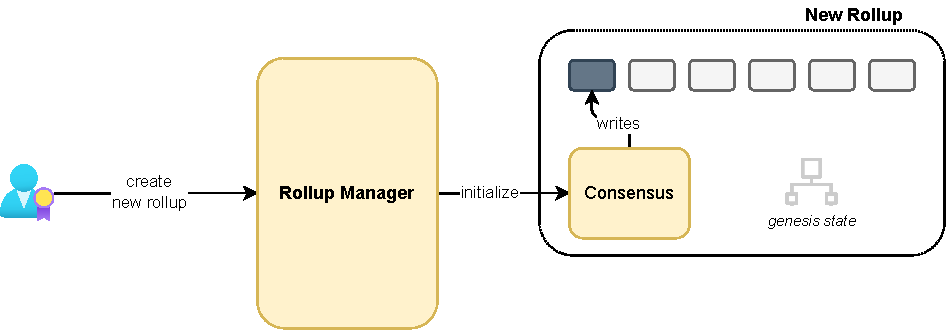
\includegraphics[width=0.8\columnwidth]{\zkevmdir/figures/architecture/ulxly/create-new-rollup.drawio}
\caption{Diagram illustrating the process of creating and initializing a new rollup instance. Observe that the state tree is empty in this situation. }
\label{fig:create-new-rollup}
\end{figure}



\paragraph*{Existing Rollups}

When an operational rollup is present on the Ethereum network, a user with the necessary rights can incorporate it into the Rollup Manager for centralized management. In this scenario, the consensus should not be initialized as the rollup, genesis block, and corresponding Bridge have already been established previously (See Figure \ref{fig:add-existing-rollup}).

\begin{figure}[h]
\centering
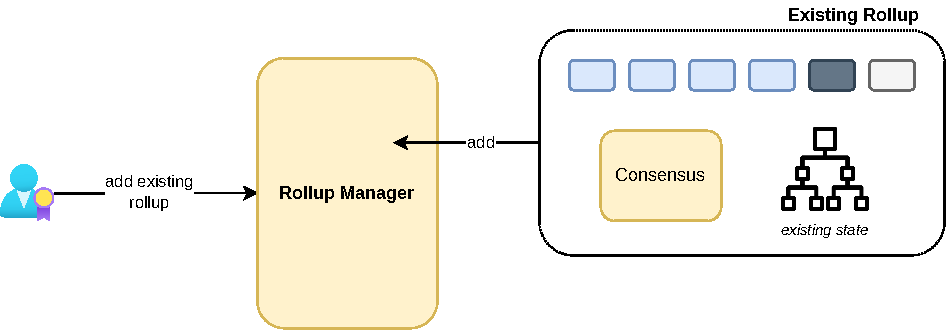
\includegraphics[width=0.6\columnwidth]{\zkevmdir/figures/architecture/ulxly/add-existing-rollup.drawio}
\caption{Diagram depicting the integration of an existing operational rollup into the Rollup Manager, showcasing the process without the need for initialization as the rollup is already established. In this case, the state tree is filled. }
\label{fig:add-existing-rollup}
\end{figure}



%%%%%%%%%%%%%%%%%%%%%%%%%%%%%%%%%%%%%%%%%%%%%%%%%%%%%%%%%%%%%%%%%%%%%%%%%%%%%%%%
\subsection{Rollup Type and Rollup Data}

\paragraph*{Rollup Type}

New rollups have a \texttt{RollupType} attached. The  \texttt{RollupType} specifies the following parameters:

\begin{itemize}
\item \textbf{The consensus implementation address}, which is the address of the contract responsible for sequencing the batches.
\item \textbf{The verifier address}, implementing the \href{https://github.com/0xPolygonHermez/zkevm-contracts/blob/develop/contracts/interfaces/IVerifierRollup.sol}{\texttt{IVerifierRollup}} interface, which allows the verification of a proof sent by the \textbf{Aggregator}.
\item \texttt{The forkID}, for tracking changes in the rollup processing.
\item \textbf{A rollup compatibility identifier}, which will be used to prevent compatibility errors when willing to \textit{upgrade} a rollup.
\item \textbf{The obsolete flag}, which is a flag for indicating whether the rollup is obsolete or not.
\item \textbf{The genesis block}, which is the initial block of the rollup and which can include a small initial state.
\end{itemize}

Note that there can be several rollups having the same \texttt{RollupType}, which means that they all share the smart contracts for consensus and batch verification. In the \texttt{RollupManager} contract, there are functions designed to add (\texttt{addNewRollupType()}) and to obsolete (\texttt{obsoleteRollupType}) rollup types. It is not possible to create rollups having an obsolete rollup type.


\paragraph*{Rollup Data}

Each rollup, apart from having a \texttt{RollupType} attached, should store some important state data, which is included in a struct called
\texttt{RollupData}. This struct contains information from the current \textbf{state} of the rollup (for example, the current batch being sequenced or verified, the states root for each batch, etc.), information of the \textbf{bridge} within the rollup (such as the current local exit root) and \textbf{forced batches} data, which will be explained in another document.

\begin{figure}[h]
\begin{solidity}
struct RollupData {

  IPolygonRollupBase rollupContract;
  uint64 chainID;
  IVerifierRollup verifier;
  uint64 forkID;

  mapping(uint64 batchNum => bytes32)              batchNumToStateRoot;
  mapping(uint64 batchNum => SequencedBatchData)   sequencedBatches;
  mapping(uint256 pendingStateNum => PendingState) pendingStateTransitions;

  bytes32 lastLocalExitRoot;
  uint64  lastBatchSequenced;
  uint64  lastVerifiedBatch;
  uint64  lastPendingState;
  uint64  lastPendingStateConsolidated;
  uint64  lastVerifiedBatchBeforeUpgrade;
  uint64  rollupTypeID;
  uint8   rollupCompatibilityID;

}
\end{solidity}
\caption{The structure definition of \texttt{RollupData} includes type information, necessary state data, bridge details, and forced batches data for a specific rollup instance.}
\label{fig:rollup-data}
\end{figure}



%%%%%%%%%%%%%%%%%%%%%%%%%%%%%%%%%%%%%%%%%%%%%%%%%%%%%%%%%%%%%%%%%%%%%%%%%%%%%%%%
\subsection{Creating a Rollup}

Each rollup is associated with either none or a single rollup type. In order to create a rollup of a certain rollup type, we can use the function \href{https://github.com/0xPolygonHermez/zkevm-contracts/blob/8fc03b0e83cbb143fdc6c1ecfaafa5c294c25509/contracts/v2/PolygonRollupManager.sol\#L559}{\texttt{createNewRollup()}} by specifying:

\begin{itemize}

\item The associated non obsolete rollup type identifier, which should exist.

\item The \texttt{chainID} of the rollup among the Polygon network, which should be new.

\item The address of the \textbf{admin} of the rollup, which will be able to update several parameters of the consensus contract (such that setting a trusted sequencer or a force batches address).

\item The address of the \textbf{trusted sequencer}, which will be the one responsible for sending the transaction to execute the \texttt{sequenceBatches()} function.

\item The address of the token address that will be used to pay gas fees in the newly created rollup (more info on this later on).

\end{itemize}

When creating a new rollup, we employ the \href{https://blog.openzeppelin.com/the-transparent-proxy-pattern}{transparent proxy pattern}, by generating an instance of the \texttt{PolygonTransparentProxy} contract, with the consensus contract specified by the rollup type serving as its implementation. The \texttt{RollupData} is \textit{partially} filled (because the rollup is not currently initialized) and stored in the \texttt{rollupIDToRollupData} mapping within the contract's storage. To end up, the rollup creation calls the \texttt{initialize()} function of the consensus, which is in charge of setting the previously specified addresses in the consensus contract.

\vspace{1em}

\begin{figure}[H]
\centering
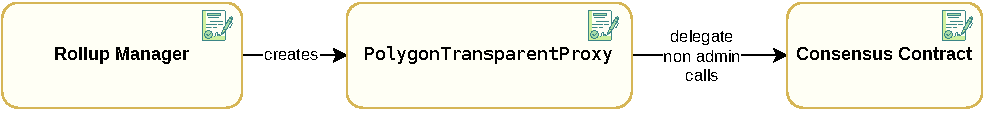
\includegraphics[width=0.85\columnwidth]{\zkevmdir/figures/architecture/ulxly/creating-new-rollup.drawio}
\caption{text}
\label{fig:transparent-proxy}
\end{figure}



\subsection{Sequencing and Verifying Flow}

\subsubsection{Sequencing Flow}

First of all, the \textbf{Sequencer} invokes the \texttt{sequenceBatches()} function within the Consensus contract to send the batches to be sequenced. Additionally, because the state information \textbf{must be stored} within the \texttt{RollupManager} contract, a callback function called \texttt{onSequenceBatches()} is triggered to store this data in the corresponding \texttt{RollupData} struct. An illustration of the sequencing flow can be found in Figure \ref{fig:consensus-flow}.

\vspace{1em}

\begin{figure}[h]
\centering
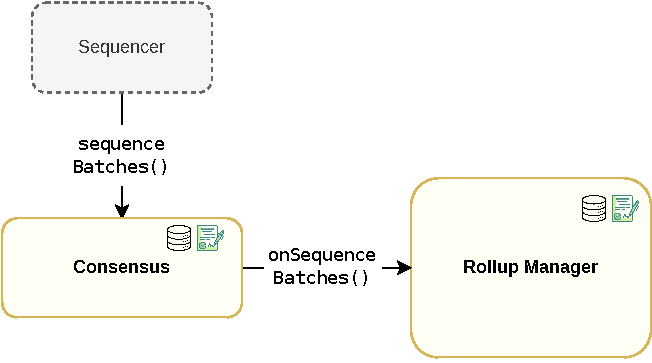
\includegraphics[width=.55\columnwidth]{\zkevmdir/figures/architecture/ulxly/ulxly-layer1-consensus-flow.drawio}
\caption{Depiction of the sequencing flow within the \textbf{Rollup Manager} component, which starts when the \textbf{Sequencer} calls the \texttt{sequenceBatches()} function. This function, in turn, invokes a callback function \texttt{onSequenceBatches()} on the \textbf{Rollup Manager} that stores the sequence data on the \texttt{RollupData} struct. }
\label{fig:consensus-flow}
\end{figure}


\subsubsection{Verifying Flow}

Once the Aggregator has constructed the corresponding proof to validate the processing of a specific set of batches, it transmits the proof for verification to the \texttt{RollupManager} by invoking the \texttt{verifyBatches()} function. Then, the \texttt{RollupManager} invokes the \texttt{veriftyProof()} function at the verifier's contract. The previous function, either validates the proof or reverts if the proof is invalid. Upon successful verification of a proof, a callback function called \texttt{onVerifyBatches()} is called in the Consensus contract. The previous function emits the \texttt{VerifyBatches} event containing important details of the processed batch such as the last verified batch. An illustration of the verifying flow can be found in Figure \ref{fig:verifier-flow}.

\vspace{1em}

\begin{figure}[h]
\centering
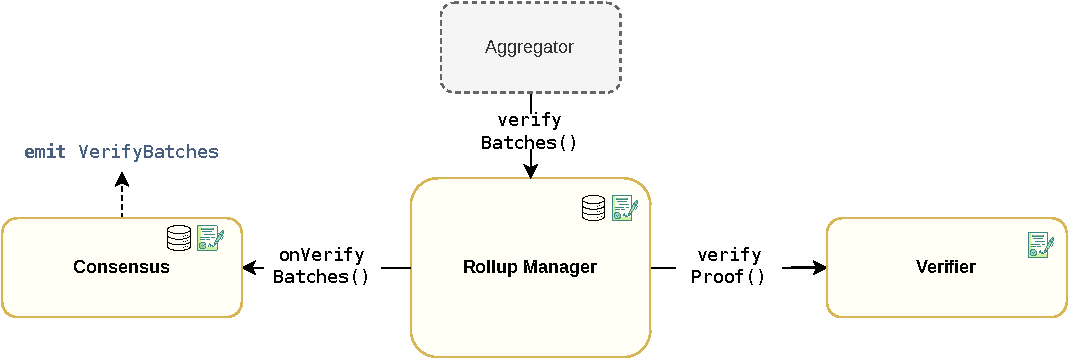
\includegraphics[width=0.8\columnwidth]{\zkevmdir/figures/architecture/ulxly/ulxly-layer1-verifier-flow.drawio}
\caption{Depiction of the verification flow within the \textbf{Rollup Manager} component, which starts when the \textbf{Aggregator} calls \texttt{verifyBatches()} function. Observe that the verification flow involves a secondary stateless \textbf{Verifier} contract, which is used in order to invoke the function \texttt{verifyProof()}. At the end of the process, the consensus emit the \texttt{verifyBatches} event. }
\label{fig:verifier-flow}
\end{figure}



%%%%%%%%%%%%%%%%%%%%%%%%%%%%%%%%%%%%%%%%%%%%%%%%%%%%%%%%%%%%%%%%%%%%%%%%%%%%%%%%
\subsection{Updating a Rollup}

This functionality provides upgradeability to the rollups. More specifically, a user with correct rights can change the consensus implementation and the rollup type of a certain rollup to modify its sequencing and/or verification procedures. In order to change the consensus, the function \texttt{UpdateRollup()} needs to change the transparent proxy implementation. In the upgrading procedure the \texttt{rollupCompatibilityID} comes into play: \textbf{in order to avoid errors, we can only upgrade to a rollup type having the same compatibility identifier as the original one}. If this is not the case, the transaction is reverted rising the \texttt{UpdateNotCompatible} error.




%%%%%%%%%%%%%%%%%%%%%%%%%%%%%%%%%%%%%%%%%%%%%%%%%%%%%%%%%%%%%%%%%%%%%%%%%%%%%%%%
\subsection{Adding Existing Rollups}


Rollups that are already deployed and already working does not follow any rollup type and are added to the \texttt{RollupManager} via the \texttt{addExistingRollup} function, specifying its current address. Meanwhile the verifier implements the \texttt{IVerifierRollup} interface we only request the raw consensus contract address, as it will not be used directly, but through a proxy to allow upgradeability options. As we have said before, we can add rollups that are deployed and already working to the \texttt{RollupManager} to allow unified management. In this case, we must call the function  \href{https://github.com/0xPolygonHermez/zkevm-contracts/blob/8fc03b0e83cbb143fdc6c1ecfaafa5c294c25509/contracts/v2/PolygonRollupManager.sol\#L640C14-L640C31}{\texttt{addExistingRollup}}.

Since the rollup has been previously initialized, we should only provide the following information:

\begin{itemize}
\item The consensus contract, implementing the \href{https://github.com/0xPolygonHermez/zkevm-contracts/blob/develop/contracts/v2/interfaces/IPolygonRollupBase.sol}{\texttt{IPolygonRollupBase}} interface.
\item The verifier contract, implementing the \href{https://github.com/0xPolygonHermez/zkevm-contracts/blob/develop/contracts/interfaces/IVerifierRollup.sol}{\texttt{IVerifierRollup}} interface.
\item The \texttt{forkID} of the existent rollup.
\item The \texttt{chainID} of the existent rollup.
\item The genesis block of the rollup.
\item The \texttt{rollupCompatibilityID}.
\end{itemize}

Observe that most of these parameters were actually provided by the \texttt{RollupType}, but existent rollups \texttt{RollupData} is constructed by hand, since they do not follow any rollup type.









%%%%%%%%%%%%%%%%%%%%%%%%%%%%%%%%%%%%%%%%%%%%%%%%%%%%%%%%%%%%%%%%%%%%%%%%%%%%%%%%
\section{Bridge within Layers}




\subsection{New Global Exit Tree}

In uLXLY, we have multiple layers, so, we need to adapt the global exit tree for storing the exits on all these layers. The design of the new global exit tree is as follows:

\begin{figure}[h]
\centering
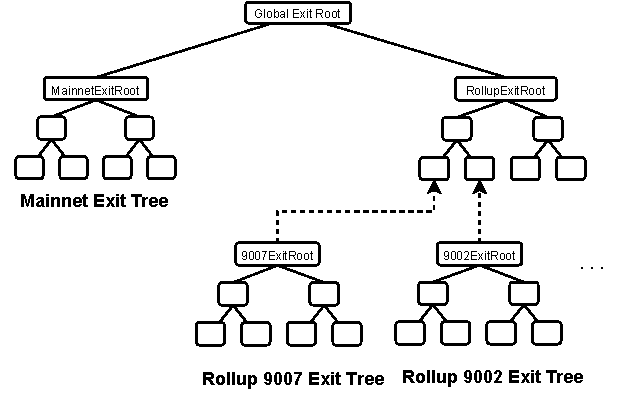
\includegraphics[width=.7\columnwidth]{\zkevmdir/figures/architecture/ulxly/ulxly-tree.drawio}
\caption{text}
\label{fig:ulxly-tree}
\end{figure}

\begin{itemize}
\item Mainnet has a local exit tree built as an append-only tree of 32 levels.
\item Each rollup, also has a local exit tree built as an append-only tree of 32 levels.
\item Rollups are grouped in a tree of rollups, that again, is built as an append-only tree of 32 levels.
\end{itemize}






\paragraph*{Rollup Identifiers.} Every rollup has a set of distinct identifiers that are essential for its functioning and interaction within the larger network ecosystem.

\begin{itemize}

\item The \texttt{chainID} is a unique identifier that distinguishes the rollup from other chains in the Ethereum ecosystem and is crucial for preventing anti-replay attacks.

\item The \texttt{networkID} identifier defines the rollup in the Polygon ecosystem, allowing network participants to uniquely identify and interact with them.

\end{itemize}

While the \texttt{networkID} convention typically begins with $1$ (because the $0$ one is reserved for mainnet), for compatibility with Merkle proof indices, its advisable to initiate counting from $0$. The rollup index (\texttt{rollupIndex}) accomplishes this goal, being $0$ when \texttt{networkID} is $1$ and similarly for higher \texttt{networkID}s.


\paragraph*{Global Index.} To create and verify the proofs, we use an index called \texttt{globalIndex} that allows to uniquely locate a leaf in the new global exit tree. The \texttt{globalIndex} consists of a string of 256 bits, with its definition starting from the most significant bit as follows:

\begin{itemize}

\item \textbf{Unused bits, 191 bits:} These bits are designated to be filled with zeros, indicating their unused status within the data structure.

\item \textbf{Mainnet Flag, 1 bit:} This single bit serves as a flag indicating whether an exit pertains to a rollup (represented by $0$) or to the mainnet (indicated by $1$).

\item \textbf{Rollup Index, 32 bits:} These bits indicate the specific rollup we are pointing to within the rollup exit tree. This bits are only used whenever mainnet flag is $0$.

\item \textbf{Local Root Index, 32 bits:} These bits indicate the specific index we are pointing to within each of the local exit trees of each rollup.

\end{itemize}

\begin{figure}[h]
\centering
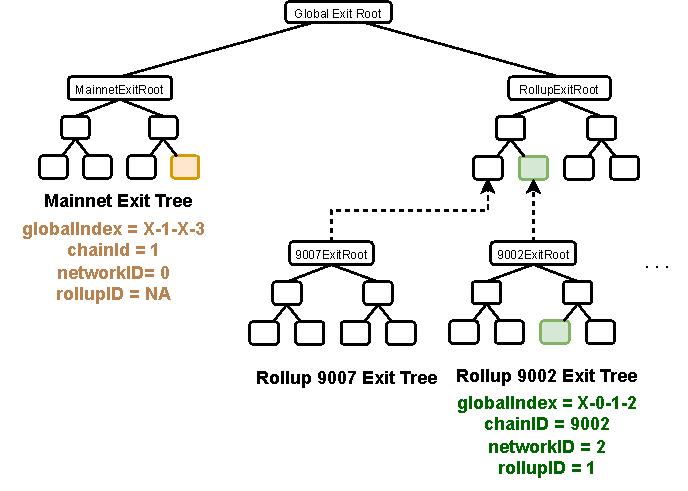
\includegraphics[width=0.8\columnwidth]{\zkevmdir/figures/architecture/ulxly/ulxly-tree-globalIndex.drawio}
\caption{This figure shows how the \texttt{globalIndex} arranges the leaves of the tree. The \texttt{globalIndex} on the left has the mainnet flag set to $1$, indicating that the bits associated with the rollup index are not utilized. Given a local root index of $11$ (equivalent to 3 in binary), we point the fourth leaf in the tree. In the right example, the mainnet flag is set to $0$. Therefore, we utilize the rollup index to find the local exit tree associated with $1$ as rollup index, which corresponds to the second leaf of the tree of rollups. Subsequently, we identify the leaf with index $10$ (equivalent to 2 in binary), which is the third leaf within the corresponding local exit tree. }
\label{fig:global-index}
\end{figure}










%%%%%%%%%%%%%%%%%%%%%%%%%%%%%%%%%%%%%%%%%%%%%%%%%%%%%%%%%%%%%%%%%%%%%%%%%%%%%%%%
\subsection{Node Configuration}

Node configuration for a rollup/validium network typically involves specifying various parameters and addresses crucial for its operation. Figure \ref{fig:node-config} provides a detailed breakdown of the parameters within the provided TOML configuration snippet.

\vspace{1em}

\begin{figure}[H]
\centering
\begin{toml}
{
    "l1Config": {
        "chainId": 1,
        "polygonZkEVMAddress": "Address of the consensus contract",
        "polygonRollupManagerAddress": "Rollup Manager SC",
        "polTokenAddress": "polTokenAddress",
        "polygonZkEVMGlobalExitRootAddress": "GlobalExitRootAddress"
    },
    "genesisBlockNumber": X,
    "root": "Initial Root of the L2 Genesis",
    "genesis": [...]
}
\end{toml}
\caption{TOML file for the node configuration of a rollup. }
\label{fig:node-config}
\end{figure}


The \texttt{chainId} is the chain identifier of the base layer (Ethereum mainnet in this case). The \texttt{genesisBlockNumber} is the L1 block number in which the rollup/validium is created.







%%%%%%%%%%%%%%%%%%%%%%%%%%%%%%%%%%%%%%%%%%%%%%%%%%%%%%%%%%%%%%%%%%%%%%%%%%%%%%%%
%\subsection{TODO: Rollup Synchronization}
%
%the l1InfoRoot mismatch:
%Nodes have to sync events from GER SC since rollup manager creation, but they only do so since rollup creation
%
%This leads to missing events -> missing leaves -> root doesnt match
%
%However, \texttt{genesisBlockNumber} seems useless (sync needs to go from the begginning of the deployment of the Rollup manager.
%
%Rollups need to have the Global Exit Tree.







%%%%%%%%%%%%%%%%%%%%%%%%%%%%%%%%%%%%%%%%%%%%%%%%%%%%%%%%%%%%%%%%%%%%%%%%%%%%%%%%

\subsection{Gas Tokens and Inter-Layer Exchanges}

The native currency to pay the \textbf{gas} at a certain layer can be:

  \begin{itemize}

  \item Any \textbf{ERC20 token} instance on any other layer.
  \item L1 ETH.

  \end{itemize}

If we use a token to pay the gas at a layer, we call this token, the \textbf{gas token} for the layer.


\begin{figure}[H]
\centering
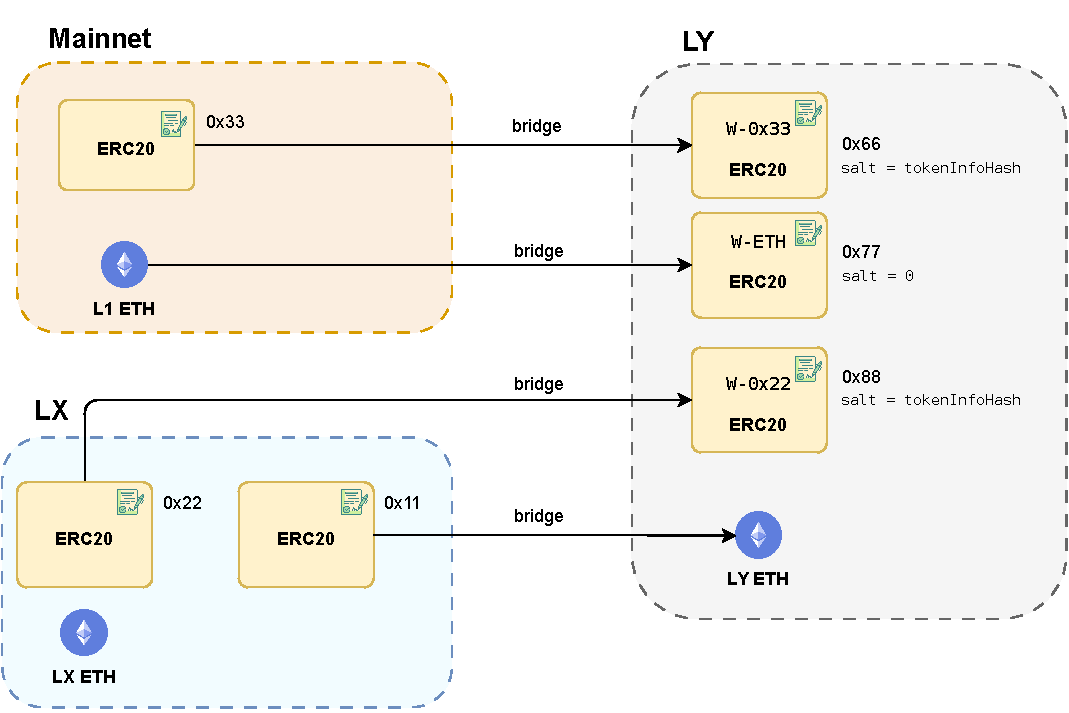
\includegraphics[width=.7\columnwidth]{\zkevmdir/figures/architecture/ulxly/ulxly-exchanges.drawio}
\caption{Diagram illustrating the interchange of assets between layers, focusing on \textbf{LY} as a layer of interest. It depicts several scenarios, such as bridging a ERC20 token from mainnet to another ERC20 token in LY, bridging L1 ETH to the LY gas token or bridging a wrapped ERC20 token living on LX to LY ETH. }
\label{fig:inter-layer-exchanges}
\end{figure}


If we are using a gas token at a layer, it is still possible to send \textbf{L1 ETH} to the layer. In this case, the ETH gets accounted in an ERC20 contract called \textbf{W-ETH}, which is just another \textbf{ERC20} instance. Note that \texttt{W-ETH} is different from the contract \texttt{WETH} (a contract for converting ETH into an ERC20 token that runs at L1 at \href{https://etherscan.io/token/0xc02aaa39b223fe8d0a0e5c4f27ead9083c756cc2\#code}{0xC02aaA39b223FE8D0A0e5C4F27eAD9083C756Cc2}). Regarding the creation of the ERC20 tokens with \texttt{CREATE2}:

\begin{itemize}
\item We use \texttt{salt = 0} to create the \texttt{W-ETH} contract.
\item We use \texttt{salt = tokenInfoHash} for the rest of the wrapped tokens of the layer with \texttt{tokenInfoHash} defined as the following hash:
\[
\texttt{tokenInfoHash} = \texttt{keccak256}(\texttt{originNetwork}, \texttt{originTokenAddress}).
\]
\end{itemize}
Finally, we would like to remark that L1 ETH is the only native currency that can be used as a native currency in another layer.


\paragraph*{Issue with the Upgradable CREATE2 Factory.}

Note that the Bridge contract is a factory of ERC20 token instances
created with \texttt{CREATE2}. Recall that \texttt{CREATE2} uses the following formula to compute the address of the instances:
\[
\texttt{instance\_address} = \texttt{hash}(\texttt{0xFF}, \texttt{sender}, \texttt{salt}, \texttt{creationBytecode}, \texttt{[args]}).
\]

Recall also that in the Bridge contract, the mapping \texttt{tokenInfoToWrappedToken} stores the addresses of all the wrapped ERC20 tokens of the layer. The \textbf{problem} is that if we \textbf{change} the \texttt{creationBytecode} of the ERC20 token contract, this will change all the addresses of the contract instances and therefore, this breaks the data of the mapping.

The \texttt{creationBytecode} will change with high probability if we compile the factory (in our case the Bridge) with another version of the Solidity compiler. In this case, we had to options:
\begin{enumerate}[a)]
\item Freeze the Solidity compiler version for the development of the whole Bridge contract.
\item Freeze the \texttt{creationBytecode} of the ERC20 token contract.
\end{enumerate}

We opted for the second solution because the ERC20 code is not prone to change so much, while freezing the compiler (and the language) for the whole Bridge could constrain its future development. Taking this approach, in the \texttt{BASE\_INIT\_BYTECODE\_WRAPPED\_TOKEN} variable of the Bridge contract you can find the pre-compiled \texttt{creationBytecode} of our ERC20 token contract.
